\pagebreak

\chapter{Anwendungsbeispiele}
Für verschiedene Einsatzszenarien sind eventuell auch verschiedene CI Lösungen die richtige Wahl, deshalb möchte ich hier ein paar Szenarien inklusive möglicher Lösungen vorstellen.
\section{Kleines Open Source Projekt mit GitHub als SCM}
Ein kleines Open Source Projekt mit nur wenigen Collaborators\footnote{Dabei handelt es sich um jemanden, der dauerhaft zu einem Projekt beiträgt und Lese- wie auch Schreibrechte auf einem GitHub Repository hat} möchte die Qualität des Codes ständig im Auge behalten. Jedoch kennt sich keiner von ihnen mit einem speziellen CI System aus. Travis-CI bietet für Open Source Projekte eine kostenlose Lösung an, bei der man lediglich eine im YAML Format erstellte Konfigurationsdatei in seinem GitHub Repository erstellen muss und eine Verbindung zu travis-ci.org herstellen. Es ist also ein einfacher Einstieg möglich, jeder kann immer auf das System zugreifen, da es im Internet gehostet wird, und es entstehen keine Kosten.\\
Ein vereinfachter schematischer Ablauf ist in \autoref{fig:Schema-Travis} zu sehen
\begin{figure}[H]
  \centering
  \fbox{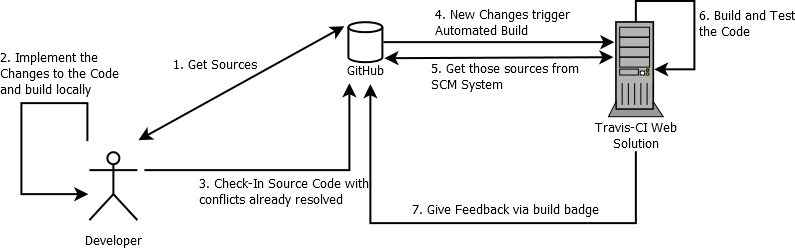
\includegraphics[width=\textwidth]{./Images/Schema-Travis.png}}
  \caption{Vereinfachter Travis-CI Prozess}\label{fig:Schema-Travis}
\end{figure}
Der Ablauf hier wurde vereinfacht dargestellt, und ähnelt in weiten Teilen dem generischen Ablauf der in \autoref{fig:Schema-aufbau} dargestellt und anschließend erklärt wurde. Es gibt bei Travis-CI neben dem möglicherweise beschränkten Zugriff auf die Builds selbst und deren Logs auch die Möglichkeit von sogenannten Badges um vom Build Ergebnis Kenntnis zu erlangen. Dies sind kleine Bilder die man einfach über die Readme.MD von GitHub in die eigene Seite einbinden kann und die das Ergebnis des Builds repräsentieren. Auf der rechten Seite in \autoref{fig:OpenConjurerFramework} ist dies zu sehen.
\begin{figure}[H]
  \centering
  \fbox{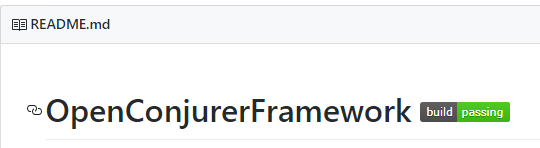
\includegraphics[width=0.5\textwidth]{./Images/OpenConjurerFramework.png}}
  \caption{GitHub Seite mit Build Badge}\label{fig:OpenConjurerFramework}
\end{figure}
\section{Mittelständisches Unternehmen aus dem Java Umfeld}
Ein mittelständisches Unternehmen möchte eine kosteneffiziente CI-Lösung einführen. Der Grund dafür ist, dass die Qualität und der Zeitraum bis zum Beheben eines kritischen Fehlers in ihrem in Java entwickelten Kernprodukt von den Kunden als mangelhaft empfunden wird. Es handelt sich dabei um ein Produkt, das keinen Regularien unterliegt und deshalb das CI System frei gewählt werden kann. Wichtigste Faktoren sind also die Verlässlichkeit und Stabilität der Lösung sowie ein möglichst geringer Kostenaufwand. Der Code soll in der eigenen Hand bleiben, da man die eigene Geistige Eigentum schützen möchte kommt nur diese Lösung in Frage. Des weiteren müssen etwa 50 bis 100 Entwickler gleichzeitig auf dem System arbeiten können.\\
Man entscheidet sich aufgrund der Rahmenbedingungen für Jenkins als CI Lösung mit mehreren dedizierten Build Agenten. Der Grund ist die große Auswahl an vorhandenen Plugins, die sehr gute Unterstützung des JAVA Entwicklungstoolings sowie das relativ einfache Skalieren. Ein mögliches solches Szenario ist in \autoref{fig:Schema-Jenkins} skizziert.
\begin{figure}[H]
  \centering
  \fbox{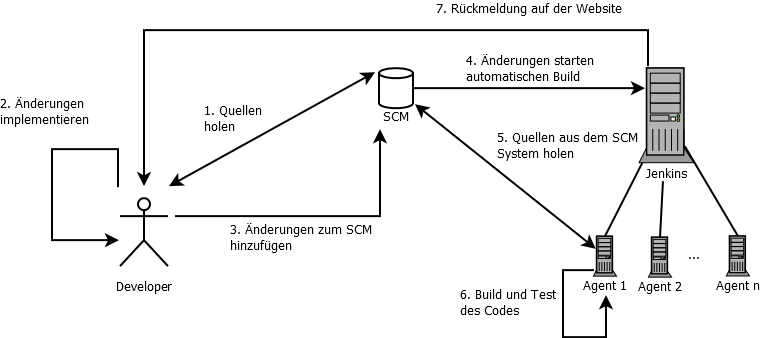
\includegraphics[width=\textwidth]{./Images/Schema-Jenkins.png}}
  \caption{Vereinfachter Jenkins Prozess mit Agents}\label{fig:Schema-Jenkins}
\end{figure}
\section{Großes Unternehmen mit Teams in unterschiedlichen Zeitzonen}
Da ich selbst als Build- \& Configurationmanager bei einem großen Unternehmen arbeite, möchte ich hier dieses System vorstellen.\\
Es handelt sich bei meinem Arbeitgeber um ein Unternehmen, das regulatorischen Rahmenbedingungen unterliegt. Des weiteren gibt es sehr viele (\~ 650) Nutzer des Systems, die sich in unterschiedlichen Zeitzonen befinden. Momentan existieren circa 1400 verschiedene Builds in unserem System. Aufgrund der schieren Menge an Aufgaben gibt es ein dediziertes Configuration Management Team mit 6 Mitarbeitern. Der Technologiestack ist hauptsächlich in der .NET Welt beheimatet und umfasst C\#, C++, C für Desktop Applikationen und Firmware sowie Java und Xamarin für Cloudservices und Apps.\\
Die Entscheidung war vor allem eine, die vom Management getrieben wurde, und es wurde TFS ausgewählt. Der Prozess umfasst mittlerweile neben CI Schritten zusätzlich nachgelagerte Tests, die auf der installierten Applikation ausgeführt werden sowie erste Release Schritte, so dass hier bereits der Übergang zu CD deutlich begonnen hat. Ein sehr reduzierter Überblick ist in \autoref{fig:Schema-Jenkins} zu sehen.
\begin{figure}[H]
  \centering
  \fbox{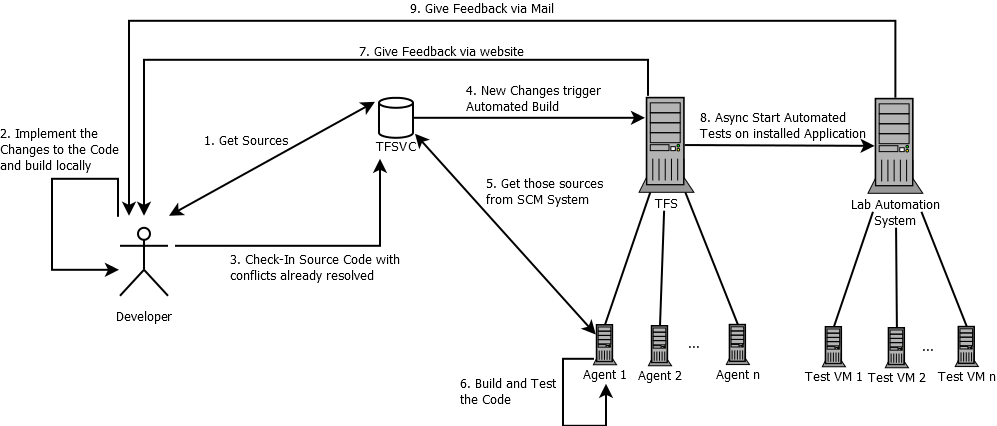
\includegraphics[width=\textwidth]{./Images/Schema-TFS.png}}
  \caption{Vereinfachter TFS Prozess mit nachgelagerten asynchronen Tests}\label{fig:Schema-TFS}
\end{figure}